\section{Theoretical analysis of the optimal deterministic policy}\label{sec:comparison}

%
%\begin{wrapfigure}{r}{0.5\textwidth}
%	\begin{center}
%    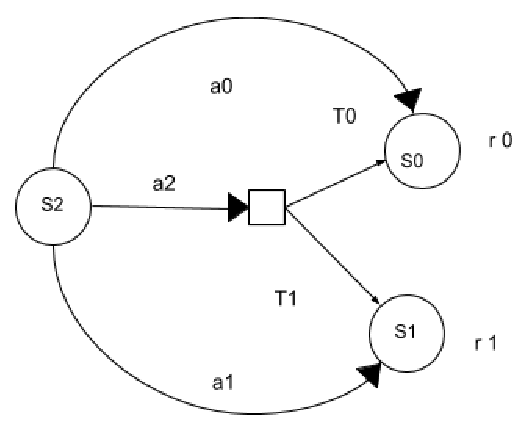
\includegraphics[scale=0.4]{images/Trident_MDP.pdf}
%	\end{center}
%	\caption{Trident IRMDP with $3$ states and $3$ actions.}
%	\label{fig:trident} 
%\end{wrapfigure}
\ET{
The goal of this section is to give a theoretical motivations of the importance of studying specific algorithms for finding an optimal deterministic policy. \\
We introduce the intuitive concept of \emph{determinising procedure}, a way to obtain a feasible deterministic policy starting from a stochastic policy. This procedure is based on the assumption that, if only one action is possible for each state, it is reasonable to assume that the most probable action should be chosen. This procedure is fast and it can be applied to any feasible stochastic policy. However, there exists no guarantee on the quality of the policy obained, regardeless of the quality of the stochastic policy used. In this section we theoretically show that using this ``common sense'' idea of adapting a stochastic policy can lead to solution signficantly suboptimal. In Section~\ref{sec:experiments} we show how the computational results obtained are consistent with the findings of this section.
%In the following two paragraphs we fist formally define the mentioned determinising procedure and subsequently we give a small example where such procedure provides a maximum regret far from the one given by the optimal deterministic policy.
}
\paragraph{\textbf{The determinising procedure.}}%\label{sec:rounding}

Let $\tilde{f}$ be a given visitation frequency value for the optimal stochastic policy. The corresponding ``rounding'' deterministic policy $\hat{\pi}$ can be computed as follows:

\begin{itemize}
\item for each $s'\in S$:
\begin{itemize}
\item find the action $a' = \text{argmax}_{a \in A}f_{s',a}$.
\item fix the rest of the action to zero: $\hat{f}_{s',a} =0, \forall a \neq a'$
\end{itemize}
\item recover the deterministic policy $\hat{\pi}$ obtained from the above fixing.
\end{itemize} 
 
The approach computes the deterministic policy by selecting the action with the highest probability for each state. Despite being pretty simple, this approach represents a plausible behaviour of a user that want to derive a deterministic policy starting from a stochastic one. 
%
%For the \textit{Tiny MDP} presented in Bruno's manuscript, it is easy to check that the rounding heuristic always gives the optimal deterministic policy (i.e., the one that minimises the max regrets).
%
%What we would like to find is a class of instances where this is not the case or, even better, instances where the difference between the heuristic deterministic policy and the optimal deterministic policy can be arbitr
%
%For a given node of the branch and 
%As bounding procedure   
%
%All the tests so far showed that the vast majority of the benders inequalities are added in the computation of the root node of the branch-and-bound (i.e., in the computation of the stochastic policy), we hope that in this way the time spent in the enumeration of the branch-and-bound tree will be reasonable.
%

\paragraph{\textbf{A small counterexample.}}%\label{sec:counter}

We define the \textit{Trident IRMDP} (see Figure~\ref{fig:trident}) as follows:
\begin{itemize}
\item Three states: $s_0, s_1, s_2$, three actions $a_0, a_1, a_2$ and a discout factor $\gamma=1$.
\item A transition function: $P(s_0 | s_2,a_0)=1$, $P(s_1 |s_2 ,a_1)=1$, $P(s_0 | s_2, a_2) = T_0$ and $P(s_1 | s_0, a_2) = T_1$.\footnote{in this formulation rewards are dependent on states. They can be easily modified to the reward function notation given in this paper $r(s, a)$} 	 
\item Two unknown rewards associated to $s_0$ and $s_1$: $r(a_0)= r_0 \in [-A,+A]$ and $r(a_1)= r_1 \in [-A+B,+A+B]$ with $A,B > 0$ and $A \gg B$. Thus, $\mathcal{R} = [-A, +A]\times[-A+B, A+B]$
\item An initial distribution on states $\beta(s_0)= \beta(s_1) = 0$ and $\beta(s_2)=1$.

\end{itemize} 

%%%%%%%%%%%%%%%%%
\begin{figure}[]
	\begin{center}
    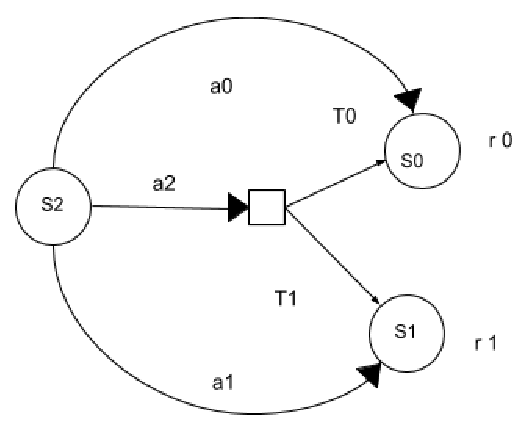
\includegraphics[scale=0.4]{images/Trident_MDP.pdf}
	\end{center}
	\caption{Trident IRMDP with $3$ states and $3$ actions.}
	\label{fig:trident} 
\end{figure}
%%%%%%%%%%%%%%%%%

The following propositions give a complete characterization of the optimal stochastic and deterministic policies for the Trident MDP. With a slight abuse of notation, we use the pedix $a$ instead of using $s_2,s_a$, i.e. instead of writing $\pi(s_2, s_a)$ we use $\pi_a$. 
%According to Figure~\ref{fig:trident}, this is due to the fact that two states $s_0$ and $s_1$ are terminal states and the only relevant actions are the ones originating from the state $s_2$ (for example, we use $\pi_1$ instead of $\pi(s_2, a_1)$). 
%For the same reason, 
We also use $r_{0}$ in place of $r(s_0)$ and $r_{1}$ in place of $r(s_1)$. Each stochastic policy on the trident MDP can be demonstrated as a tuple $\pi = (\pi_0, \pi_1, \pi_2)$. %where each element indicates the probability of choosing action $a_i$ in state $s_i$. 
Similarly, the visitation frequency functions are presented as $f = (f_0, f_1, f_2)$.

\begin{proposition}\label{theorem:opt_stoc}
An optimal stochastic policy that minimises the maximum regret (see Section~\ref{sec:Preliminaries}) for the Trident MDP is the policy $\tilde{\pi} = (\pi_0, \pi_1, \pi_2)$ defined as:
$$\pi_{0}=\dfrac{2A - B}{4A},~~~\pi_{1}=\dfrac{2A + B}{4A}, ~~~\pi_2 = 0\;.$$
%(regardless of the values of $T_1$ and $T_2$). \footnote{We recall that $\pi_0$ means $\pi(s_2, a_0)$ and so on.}
\end{proposition}
\begin{proof}
%We first show that there exists always an optimal stochastic policy with $\pi_2 = 0$. We do this by
We first observe that for every policy $\pi' = (\pi'_0, \pi'_1, \pi'_2)$ with $\pi'_2 > 0$, it is possible to construct a policy $\pi'' = (\pi''_0, \pi''_1, \pi''_2)$ with $\pi''_2 = 0$ and with the same value in the following way:
\begin{align*}
\pi''_0 = \pi'_0 + \pi'_2 T_0, ~~~ \pi''_1 = \pi'_1 + \pi'_2 T_1\;.
\end{align*}
If we compute the value of the first policy we notice that:
\begin{align*}
\beta \cdot V^{\pi'} = V^{\pi'}(s_2) =
r_{_0} \pi'_0 + r_{_1}\pi'_1 + r_{_0} T_0 \pi'_2 + r_{_1} T_1 \pi'_2 \\
= r_{_0} (\pi'_0 + T_0 \pi'_2) + r_{_1} (\pi'_1 + T_1 \pi'_2)
= r_{_0} \pi''_0 + r_{_1}\pi''_1  \\
= V^{\pi''}(s_2) =\beta \cdot V^{\pi''}\;,
\end{align*}
showing that both policies have the same value.
Moreover, the equivalence shows that  $\beta \cdot V^{\pi'}= \beta \cdot V^{\pi''}$, $\forall r \in \mathcal{R}$,
this implies that
$\pi'$ and $\pi''$ have equivalent maximum regret, because: $MR(\pi', \mathcal{R}) = \text{max}_{r} \text{max}_g r \cdot g - \beta \cdot V^{\pi'} = \text{max}_{r} \text{max}_g r \cdot g - \beta \cdot V^{\pi''} = MR(\pi'', \mathcal{R})$.
% indicates that for each stochastic policy there exists a stochastic policy with the same value but with $\pi_2 = 0$. 
We can hence suppose that there exists an optimal stochastic policy with $\pi_2 =0$ as a solution for minimax regret. 

As second part of the proof, we compute the value of the optimal policy considering $\tilde{\pi} = (\pi_0, \pi_1, 0)$ where $\pi_0, \pi_1 \geq 0$ similarly its equivalent visitation frequency is $\tilde{f} = (f_0, f_1, 0)$. 
%Let $\pi_0,\pi_1$ be a generic policy. 
We notice that the adversary policy by its equivalent visitation frequency $g$ giving a maximum regret is always deterministic (see~\ref{sec:Preliminaries}). For this reason, we have only two adversary policies: we can have either $g = (g_0, g_1, g_2)$ where $g_0 = g_2=0$ and $g_1 > 0$ or the opposite, $g' = (g_0, g_1, g_2)$ where $g_0>0$ and $g_1 = g_2 = 0$. (We notice that, with arguments analogous to the ones used in the first part of the proof, we can rule out the case where $g_2 \geq 0$.)

Knowing that the maximum regret is the maximum among two choices for the adversary policies, the maximum regret associated to the policy $g =(0, g_1, 0)$ (obtained by fixing $r_0 = -A$ and $r_1 = A+B$) is the following
\begin{align}
r \cdot g - r \cdot \tilde{f} = A + B +A \pi_0 -(A+B)\pi_1 \label{eq:best_stoc_1}
\end{align}   
and the maximum regret associated to the policy $g' = (g_0, 0, 0)$ where $g_0 > 0$ is obtained by fixing $r_0 = A$ and $r_1 = -A+B$, leading to a value of
\begin{align}
r \cdot g - r \cdot \tilde{f}  = A - A \pi_0 -(B-A)\pi_1 \label{eq:best_stoc_2}\;.
\end{align}   
We are interested in minimising the max regret, this means that we want to find the values of $\pi_0$ and $\pi_1$ that minimise $\max \{\eqref{eq:best_stoc_1}, \eqref{eq:best_stoc_2}\}$. The optimal stochastic policy can hence be obtained by solving the following system of two equations: 
\begin{align*}
A + B +A \pi_0 -(A+B)\pi_1 &= A - A \pi_0 -(B-A)\pi_1\\
\pi_0+\pi_1 &= 1
\end{align*} 
That has as optimal solution the values $\pi_{0}=\dfrac{2A - B}{4A}$ and $\pi_{1}=\dfrac{2A + B}{4A}$, concluding the proof.
\end{proof}


Proposition~\ref{theorem:opt_stoc} implies the following Lemma:
\begin{lemma}\label{lemma:heur_policy}
The determinised policy for the Trident MDP is $\hat{\pi} = (0, 1, 0)$ %$ $\pi_0 =\pi_2 = 0$ and $\pi_1 = 1$ 
and its maximum regret is $MR(\hat{f}, \mathcal{R}) = 2A-B$.
\end{lemma}
\begin{proof}
It is a direct consequence of the fact that in the optimal stochastic policy we always have $\pi_1 > \pi_2$ and $\pi_0 = 0$.
\end{proof}

\begin{proposition}\label{theorem:opt_det}
If $T_1 > T_0$, the optimal deterministic policy is $\pi^* = (0, 0, 1)$ and its maximum regret is $MR(f^*, \mathcal{R}) = A- A T_0 +(A-B) T_1$. 
\end{proposition}
\begin{proof}
We prove the statement by explicitly computing the maximum regret of the three possible deterministic policies:$\pi = (1, 0, 0), \pi' =(0, 1, 0), \pi''= (0, 0, 1)$ $\pi_0=1$.

\textit{Maximum regret of $\pi = (1, 0, 0)$}. We want to find the adversary policy that maximises the regret for the policy $\pi$. We do that by computing all possible combinations of adversary policies and rewards:
\begin{itemize}
\item If a visitation frequency for adversary policy is $g = (0, g_1, 0)$ where $g_1> 0$, the reward maximising the regret is $r_0 = -A$ and $r_1 = A+B$, leading to a maximum regret of 

\begin{align}
A+B-(-A)=2A+B \label{eq:regret0}
\end{align}
\item If the adversary policy is $g' = (0, 0, g_2)$ where $g_2>0$, we need to check all four combinations of extreme rewards:
\begin{itemize}
\item $r_0 = -A$ and $r_1= A+B$. Maximum regret of
\begin{align}
-A T_0 + (A+B)T_1 + A = (1-T_0 + T_1)A + T_1 B \label{eq:regret1}
\end{align}
\item $r_0 = A$ and $r_1= A+B$. Maximum regret of
\begin{align}
A T_0 + (A+B)T_1 - A = (-1+T_0 + T_1)A + T_1 B  \label{eq:regret2}
\end{align}
\item $r_0 = A$ and $r_1= -A+B$. Maximum regret of
\begin{align} 
A T_0 + (-A+B)T_1 - A =  (-1+T_0 - T_1)A + T_1 B \label{eq:regret3}
\end{align}
\item $r_0 = -A$ and $r_1= -A+B$. Maximum regret of
\begin{align}
-A T_0 + (-A+B)T_1 + A =  (1 - T_0 - T_1)A - T_1 B \label{eq:regret4}
\end{align}
\end{itemize} 
By hypothesis we have that $A\gg B$ and $T_0+T_1= 1$, this implies that $\eqref{eq:regret0} \geq \max\{\eqref{eq:regret1}, \eqref{eq:regret2}, \eqref{eq:regret3}, \eqref{eq:regret4} \}$. Therefore, the maximum regret if $g_2>0$ is $MR(f^{\pi}, \mathcal{R}) = 2A+B$.
\end{itemize} 

\textit{Maximum regret of $\pi' = (0, 1, 0)$}.
It is trivial to check, with calculations analogous to the one used above to compute the regret of $\pi$, that the maximum regret in this case is equal to $MR(f^{\pi'}, \mathcal{R}) = 2A-B$.


\textit{Maximum regret of $\pi'' = (0, 0, 1)$}.
Also in this case, we need to consider the two cases of $g =(g_0, 0 ,0)$ where $g_0 > 0$ and $g' = (0, g_1, 0)$ with $g_1 > 0$. For $g$, we fix $r_0 = A$ and $r_1 = -A+B$, obtaining a regret equal to 
\begin{align}
A- A T_0 +(A-B) T_1 \label{eq:regret2_1}
\end{align}
And for $g'$ we fix $r_0 = -A$ and $r_1 = A+B$, obtaining a regret equal to 
\begin{align}
A+B+A T_0 -(A+B) T_1\;. \label{eq:regret2_2}
\end{align}
The maximum between~\eqref{eq:regret2_1} and~\eqref{eq:regret2_2} depends on the values of $T_0$ and $T_1$.
By imposing  $A- A T_0 +(A-B) T_1 \geq A+B+A T_0 -(A+B) T_1$ we obtain:
$$ 2A T_1 \geq 2 A T_0 + B\;. $$
We recall that by construction we have $A \gg B$, this implies that if $T_1> T_0$ (resp. $T_1\leq T_0$)  we have that the maximum regret is equal to~\eqref{eq:regret2_1} (resp.~\eqref{eq:regret2_2}).
The minimum maximum regret found so far is the one obtained for $\pi = \pi' = (0, 1, 0)$, and it is equal to $MR(f^{\pi'}, \mathcal{R}) = 2A-B$. Therefore, it remains to check for which values of $T_0 > T_1$ we have that $2A-B \geq~\eqref{eq:regret2_1}$:
\begin{align*}
A- A T_0 +(A-B) T_1 \leq 2A - B \\
 \Leftrightarrow A- A (1-T_1) +(A-B) T_1 \leq 2A - B\\
  \Leftrightarrow (2A-B)T_1 \leq 2A-B  \Leftrightarrow T1 \leq 1\;.
\end{align*}
 Since we have by construction that $T_1 \leq1$ we can conclude that for any $T_1> T_0$ the optimal deterministic policy is $\piç* = \pi''= (0, 0,1)$ and its maximum regret is equal to $MR(f^{\pi''}, \mathcal{R})A- A T_0 +(A-B) T_1$. 
\end{proof}

Proposition~\ref{theorem:opt_det} and Lemma~\ref{lemma:heur_policy} shows that for any Trident MDP we have that the optimal deterministic policy and the rounding deterministic policy are always different. 


The following Lemma shows that the rounding policy could be significantly worse than the optimal deterministic policy:

\begin{lemma}\label{lemma:gap2}
The ratio between the maximum regret of the determinised policy and the optimal deterministic policy goes to $2$ with the increase of the value of $A$ with respect to $B$ and the increase of $T_1$. In other words:  
\begin{align*}
\lim_{A/B \rightarrow \infty, T_1 \rightarrow {\frac{1}{2}}^+} \dfrac{2A-B}{A- A T_0 +(A-B) T_1} = 2
\end{align*}
\end{lemma}
\begin{proof}
The statement follows from the definition of the limit.
\end{proof}

%Lemma~\ref{lemma:gap2} shows that even small MDP can present

From a theoretical point of view, it is still unknown what is the highest possible value we can have greater than $2$ (or even a ratio that goes to infinity). From a practical point of view, such small example shows how the use of the determinising policy can lead to a maximum regret  $100\%$ far from the optimal. 